\begin{figure}[htbp]
    \begin{center}
        \subfigure[Resultados de aptitud para el experimento]{%
            \label{fig:exp3_first}
            %\scalebox{0.8}{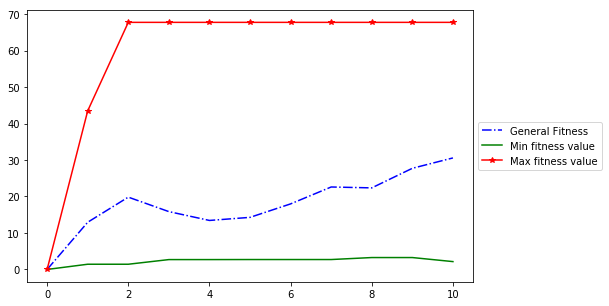
\includegraphics[width=0.8\textwidth]{Fitness.png}}
            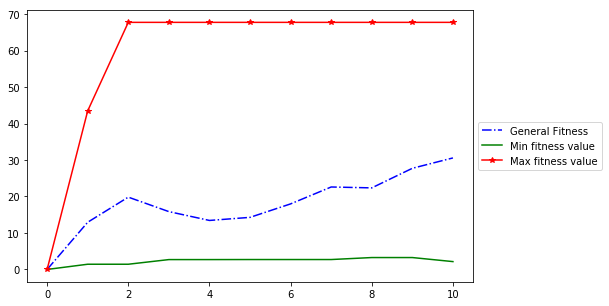
\includegraphics[width=0.6\textwidth]{Fitness.png}
        }\\%
        %\subfigure[Distancia Hamming promedio en el experimento]{%
        %\label{fig:second}
        %\scalebox{0.8}{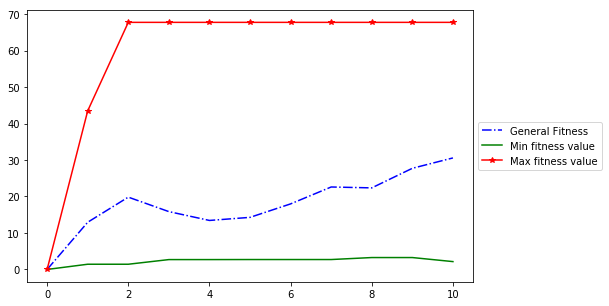
\includegraphics[width=0.8\textwidth]{Fitness.png}}
        %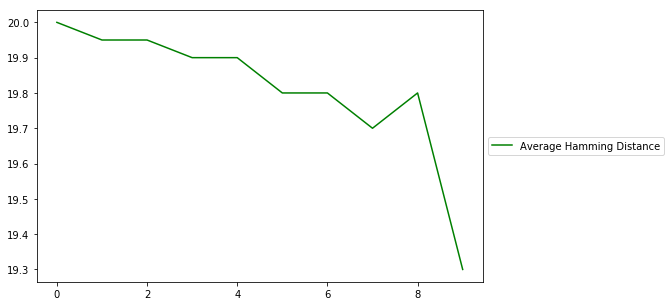
\includegraphics[width=0.6\textwidth]{Hamming.png}
        %}\\ 
            
        %  ------- End of the first row ----------------------%
        \subfigure[Mejor individuo, generación 1]{%
            \label{fig:exp3_third}
            \scalebox{1.8}{\begin{tikzpicture}
\node at (0,2) {
\includegraphics[width=3cm, trim={0 0 0 60}, clip]{Gen1Ind1_BF.PNG}};
\node at (0,0) {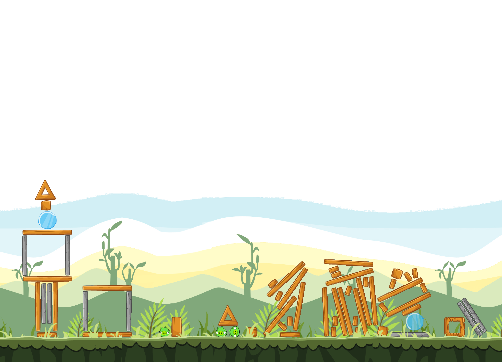
\includegraphics[width=3cm, trim={0 0 0 60}, clip]{Gen1Ind1_AF.PNG}};
%\node[rotate=30] at (1,2) {\includegraphics[width=3cm]{example-image}};
\end{tikzpicture}}
            %\scalebox{2.0}{\begin{tikzpicture}
\node at (0,2) {
\includegraphics[width=3cm, trim={0 0 0 60}, clip]{Gen1Ind1_BF.PNG}};
\node at (0,0) {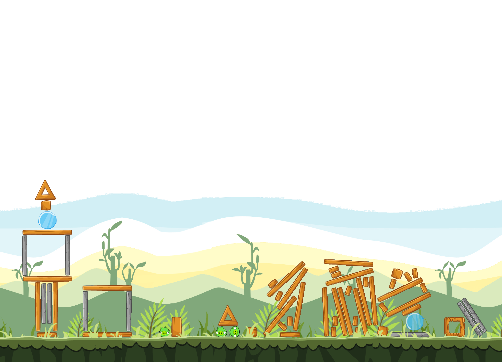
\includegraphics[width=3cm, trim={0 0 0 60}, clip]{Gen1Ind1_AF.PNG}};
%\node[rotate=30] at (1,2) {\includegraphics[width=3cm]{example-image}};
\end{tikzpicture}}
        }%
        \subfigure[Peor individuo, generación 1]{%
            \label{fig:exp3_fourth}
            \scalebox{1.8}{\begin{tikzpicture}
\node at (0,3) {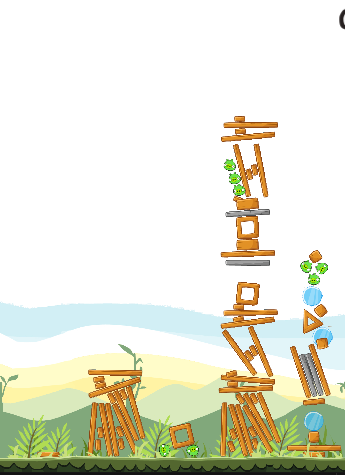
\includegraphics[width=3cm, trim={0 0 5 10}, clip]{Gen1Worst_Before.PNG}};
\node at (0,0) {
\includegraphics[width=3cm, trim={0 0 0 60}, clip]{Gen1Worst_After.PNG}};
%\node[rotate=30] at (1,2) {\includegraphics[width=3cm]{example-image}};
\end{tikzpicture}}
        }
    \end{center}
    \caption{Resultados del experimento, grafica de la función de aptitud figura a), ejemplos de individuos: figuras b) y c)}
    \label{figure:exp_03_a}
\end{figure}
%\newpage
\begin{figure}[htbp]
    \begin{center}
    %
        \subfigure[Mejor individuo, ultima generación]{%
            \label{fig:exp3_fifth}
            \scalebox{2.2}{\begin{tikzpicture}
\node at (0,2) {
\includegraphics[width=3cm, trim={0 0 0 60}, clip]{Last_Gen_1st_Best_Before.PNG}};
\node at (0,0) {
\includegraphics[width=3cm, trim={0 0 0 60}, clip]{Last_Gen_1st_Best_After.PNG}};
%\node[rotate=30] at (1,2) {\includegraphics[width=3cm]{example-image}};
\end{tikzpicture}}
        }\\%
        \subfigure[Segundo mejor individuo, ultima generación]{%
            \label{fig:exp3_sixth}
            \scalebox{2.1}{\begin{tikzpicture}
\node at (0,2) {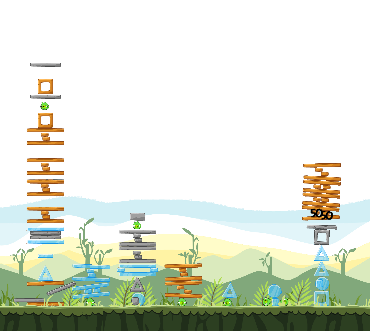
\includegraphics[width=3cm, trim={0 0 0 60}, clip]{Last_Gen_2nd_Best_Before.PNG}};
\node at (0,0) {
\includegraphics[width=3cm, trim={0 0 0 60}, clip]{Last_Gen_2nd_Best_After.PNG}};
%\node[rotate=30] at (1,2) {\includegraphics[width=3cm]{example-image}};
\end{tikzpicture}}
        }%
        % 
    \end{center}
    \caption{Resultados del experimento, primer y segundo mejor nivel generado (sin repetir)}
    \label{figure:exp_03_b}
\end{figure}
